\documentclass{fenicsmanual}

\begin{document}

\fenicstitle{DOLFIN User Manual}
\fenicsauthor{Hoffman, Jansson, Logg, Wells}
\fenicspackage{\textbf{\textsf{DOLFIN}}}{dolfin}
\fenicsimage{eps/dolfin.eps}

\maketitle

% This chapter is common to the DOLFIN and FFC manuals.

\addcontentsline{toc}{chapter}{About this manual}
\chapter*{About this manual}

This manual is currently being written. A first version of this manual
should be ready sometime in the fall of 2005.

%------------------------------------------------------------------------------
\section*{Intended audience}

This manual is written both for the beginning and the advanced user.
There is also some useful information for developers. More advanced topics
are treated at the end of the manual or in the appendix.

%------------------------------------------------------------------------------
\section*{Typographic conventions}

\begin{itemize}
\item
  Code is written in monospace (typewriter) \texttt{like this}.
\item
  Commands that should be entered in a Unix shell
  are displayed as follows:
  \begin{code}
    # ./configure
    # make
  \end{code}
  Commands are written in the dialect of the \texttt{bash} shell. For
  other shells, such as \texttt{tcsh}, appropriate translations may be
  needed.
\end{itemize}

%------------------------------------------------------------------------------
\section*{Contact}

Comments, corrections and contributions to this manual are most welcome
and should be sent to
\begin{code}
  \packagett{}-dev@fenics.org    
\end{code}

%\chapter{Introduction}

\fixme{Automation of CMM, FEniCS, purpose of DOLFIN: PSE for differential equations, C++ interface of
  FEniCS, etc}

%------------------------------------------------------------------------------
\section{The FEniCS project}

\fixme{Automation of CMM, other components of \fenics{}}

%------------------------------------------------------------------------------
\section{The finite element method}

\fixme{Automation of discretization}

%------------------------------------------------------------------------------
\section{Overview}

\fixme{Component diagram, user, module, kernel}

\input{chapters/quickstart.tex}
\input{chapters/linearalgebra.tex}
\chapter{The mesh}

\fixme{Triangular, tetrahedral, include some images, mesh refinement, connectivity, iterators, file formats, local ordering}

\input{chapters/functions.tex}
\chapter{Ordinary differential equations}

\devnote{This chapter needs to be written. In the meantime, checkout the demos
  in \texttt{src/demo/ode/} and the base class \texttt{ODE}.}


% FIXME: Mono-adaptive, multi-adaptive, ODE base class, simple example,
% FIXME: error control, adaptivity, complex ODE, implicit, homotopies

\chapter{Partial differential equations}

\section{Variational formulation}

Bilinear form, linear form, FFC

\section{Finite elements}

Finite Element by Ciarlet, FIAT 

\section{Element matrices and vectors} 

divide element matrix into geometry tensor and integration 
over reference element FErari

precomputation of integrals, quadrature, tensorrepresentation factored out, FFC 

\section{Assembly}

dofs, vector dofs, 

\section{Functionals}

postprocess FFC 

\fixme{Variational formulation, examplify with Poisson, FFC, finite elements, FIAT, assembly, functionals}

% Insert note that constants are passed into forms as references

\chapter{Nonlinear solver}
\index{nonlinear solver}

\devnote{This chapter is currently being written\ldots}

\dolfin{} provides tools for solving nonlinear equations of the form
\begin{equation}
  F(u) = 0
\end{equation}
where $F: \mathbb{R}^{n} \rightarrow \mathbb{R}^{n}$. The nonlinear solvers are
based on Newton's method and utilise functions from PETSc \cite{www:petsc}.    

To use the nonlinear solver, a nonlinear function must be defined. The nonlinear
solver is then initialised with this function and a solution computed.



\section{Nonlinear functions}
\index{NonlinearFunction}

To solve a nonlinear problem, the user must defined a class which . The class 
should be derived from the \dolfin class \texttt{NonlinearFunction}. The class 
should contain the necessary functions to form the function $F(u)$ and the 
Jacobian matrix  $J = \partial F / \partial u$. The precise form of the user 
defined class will depend on the PDE being solved and the numerical method.
The structu of a user defined class \texttt{MyNonlinearFunction} is shown below.
\begin{code}
class MyNonlinearFunction : public NonlinearFunction
\{
  public: 
  
    // Constructor 
    MyNonlinearFunction() : NonlinearFunction()\{\}
  
    // Compute F(u) 
    void F(Vector\& b, const Vector\& x)
    \{
      // Insert F(u) into the vector b 
    \}

    // Compute J
    void J(Matrix\& A, const Vector\& x)
    \{
      // Insert the Jacobian into the matrix A 
    \}

    dolfin::uint size()
    \{      
      // Return the dimension of the Jacobian matrix 
    \}

    dolfin::uint nzsize()
    \{      
      // Return the maximum number of zeroes per row of the Jacobian
    \}

  private:
    // Pointers to objects with which F(u) is defined
\};
\end{code}


\section{Newton solver}
\index{Newton's method}
\index{NewtonSolver}

\subsection{Linear solver}

\subsection{Application of Dirichlet boundary conditions}

The application of inhomogenuous Dirichlet boundary conditions in the context
of a Newton solver requires particular attention.



\subsection{Newton solver parameters}

\subsection{Application of Dirichlet boundary conditions}


\section{Incremental Newton solver}


\input{chapters/io.tex}
\chapter{The log system}

\dolfin{} provides provides a simple interface for uniform handling of
log messages, including warnings and errors. All messages are
collected to a single stream which allows the destination and
formatting of the output from a entire program, including the
\dolfin{} library, to be controlled by the user.

%------------------------------------------------------------------------------
\section{Generating log messages}

Log messages can be generated using the function
\texttt{dolfin\_info()} available in the \texttt{dolfin} namespace:
\begin{code}
  void dolfin_info(const char *msg, ...);
\end{code}
which works similarly to the standard C library function \texttt{printf}.
The following examples illustrate the usage of
\texttt{dolfin\_info()}:
\begin{code}
  dolfin_info(``Solving linear system.'');
  dolfin_info(``Size of vector: \%d.'', x.size());
  dolfin_info(``R = \%.3e (TOL = \%.3e)'', R, TOL);
\end{code}

As an alternative to \texttt{dolfin\_info()}, \dolfin{} provides a C++
style interface to generating log messages. Thus, the above examples
can also be implemented as follows:
\footnotesize
\begin{code}
  cout << ``Solving linear system.'' << endl;
  cout << ``Size of vector: `` << x.size() << ``.'' << endl;
  cout << ``R = `` << R << `` (TOL = `` << TOL << ``)'' << endl;
\end{code}
\normalsize
using \texttt{dolfin::cout} and \texttt{dolfin::endl} from the \texttt{dolfin}
namespace, corresponding to the standard standard \texttt{std::cout}
and \texttt{std::endl} in namespace \texttt{std}. If log messages are
directed to standard output (see below), then \texttt{dolfin::cout}
and \texttt{std::cout} may be mixed freely.

%------------------------------------------------------------------------------
\section{Warnings and errors}

Warnings and error messages can be generated using the macros
\begin{code}
  dolfin_warning(message);
  dolfin_error(message);
\end{code}

In addition to displaying the given string message, the macro
\texttt{dolfin\_error()} also displays information about the location
of the code that generated the error (file, function name and line
number). Once an error is encountered, the program is stopped.

Note that in order to pass formatting strings and additional arguments
to warnings or errors, the variations \texttt{dolfin\_error1()},
\texttt{dolfin\_error2()} and so on must be used, as illustrated by
the following examples:
\footnotesize
\begin{code}
  dolfin_error(``GMRES solver did not converge.'');
  dolfin_error1(``Unable to find face opposite to node %d.'', n);
  dolfin_error2(``Unable to find edge between nodes %d and %d.'', n0, n1);
\end{code}
\normalsize

%------------------------------------------------------------------------------
\section{Debug messages and assertions}

The macro \texttt{dolfin\_debug()} works similarly to
\texttt{dolfin\_info()}:
\begin{code}
  dolfin_debug(message);
\end{code}
but in addition to displaying a message, information is printed about
the location of the code that generated the debug message (file,
function name and line number).

Note that in order to pass formatting strings and additional arguments
with debug messages, the variations \texttt{dolfin\_debug1()},
\texttt{dolfin\_debug2()}, depending on the number of arguments.

Assertions can often be a helpful programming tool. Use assertions
whenever you assume something about about a variable in your code,
such as checking that given input to a function is valid. \dolfin{}
provides the macro \texttt{dolfin\_assert()} for creating assertions:
\begin{code}
  dolfin\_assert(check);
\end{code}
This function accepts a boolean expression and if the expression
evaluates to false, an error message is displayed, including the
file, function name and line number of the assertion, and a
segmentation fault is raised (to enable easy attachment to a
debugger). The following examples illustrate the use of
\texttt{dolfin\_assert()}:
\begin{code}
  dolfin_assert(i >= 0);
  dolfin_assert(i < n);
  dolfin_assert(cell.type() == Cell::triangle);
  dolfin_assert(cell.type() == Cell::tetrahedron);
\end{code}
Note that assertions are only active if \dolfin{} when compiling
\dolfin{} and your program with \texttt{DEBUG} defined (configure
option \texttt{--enable-debug} or compiler flag \texttt{-DDEBUG}).
Otherwise, the macro \texttt{dolfin\_assert()} expands to nothing,
meaning that liberal use of assertions does not mean a performance
penalty, since assertions only are present during development and
debugging.

%------------------------------------------------------------------------------
\section{Task notification}

The two function \texttt{dolfin\_begin()} and \texttt{dolfin\_end()}
available in the \texttt{dolfin} name space can be used to notify the
\dolfin{} log system about the beginning and end
The \dolfin{} log system indents log messages hierarchically 
To notify the \dolfin{} log system about the beginning of 
\dolfin{} provides two functions 
%// Task notification
%namespace dolfin { void dolfin_begin(); }
%namespace dolfin { void dolfin_begin(const char* msg, ...); }
%namespace dolfin { void dolfin_end(); }
%namespace dolfin { void dolfin_end(const char* msg, ...); }

%------------------------------------------------------------------------------
\section{Progress bars}
\index{progress bar}

To notify progress by a progress session, use the class
Progress.

Examples of usage:

\begin{code}
  Progress p("Assembling", grid.noCells());
  
  for (CellIterator c(grid); !c.end(); ++c) {
    ...
    p++;
  }
\end{code}

Progress also supports the following usage:

\begin{code}
  p = i;    // Specify step number
  p = 0.5;  // Specify percentage
  p.update(t/T, "Time is t = %f", t);
\end{code}

%------------------------------------------------------------------------------
\section{Controlling the destination of output}

% curses, terminal, silent
%
% // Update (force refresh of curses interface)
% namespace dolfin { void dolfin_update(); }
%
%
%// Specify output type (``plain text'', ``curses'', or ``silent'')
%void dolfin_output(const char* type);
%
%// Switch logging on or off
%void dolfin_log(bool state);




\chapter{Parameters}
\index{parameters}

\dolfin{} keeps a global database of parameters that control the
behavior of the various components of \dolfin{}. Parameters are
controlled using a uniform type-independent interface that allows
retrieving the values of existing parameters, modifying existing
parameters and adding new parameters to the database.

%------------------------------------------------------------------------------
\section{Retrieving the value of a parameter}
\index{\texttt{dolfin\_get()}}

To retrieve the value of a parameter, use the function \texttt{dolfin\_get()}
available in the \texttt{dolfin} namespace:
\begin{code}
  Parameter dolfin_get(const char* key);
\end{code}
This function accepts as argument a string \texttt{key} and returns
the value of the parameter matching the given key. An error message is
printed through the log system if there is no parameter with the given
key in the database.

The value of the parameter is automatically cast to the correct type
when assigning the value of \texttt{dolfin\_get()} to a variable, as
illustrated by the following examples:
\begin{code}
  real TOL = dolfin_get(``tolerance'');
  int num_samples = dolfin_get(``number of samples'');
  bool solve_dual = dolfin_get(``solve dual problem'');
  std::string filename = dolfin_get(``file name'');
\end{code}

Note that there is a cost associated with accessing the value of a
parameter, so if the value of a parameter is to be used multiple
times, then it should be retrieved once and stored in a local variable
as illustrated by the following example:
\begin{code}
  int num_samples = dolfin_get(``number of samples'');
  for (int i = 0; i < num_samples; i++)
  \{
    ...
  \}
\end{code}

%------------------------------------------------------------------------------
\section{Modifying the value of a parameter}
\index{\texttt{dolfin\_set()}}

To modify the value of a parameter, use the function \texttt{dolfin\_set()}
available in the \texttt{dolfin} namespace:
\begin{code}
  void dolfin_set(const char* key, ...);
\end{code}
This function accepts as arguments a string \texttt{key} together with
the corresponding value. The value type should match the type of
parameter that is being modified. An error message is
printed through the log system if there is no parameter with the given
key in the database.

The following examples illustrate
the use of \texttt{dolfin\_set()}:
\begin{code}
  dolfin_set(``tolerance'', 0.01);
  dolfin_set(``number of samples'', 10);
  dolfin_set(``solve dual problem'', true);
  dolfin_set(``file name'', ``solution.xml'');
\end{code}

Note that changing the values of parameters using
\texttt{dolfin\_set()} does not change the values of already retrieved
parameters; it only changes the values of parameters in the
database. Thus, the value of a parameter must be changed before using
a component that is controlled by the parameter in question.

%------------------------------------------------------------------------------
\section{Adding a new parameter}
\index{\texttt{dolfin\_parameter()}}

To add a parameter to the database, use the function
\texttt{dolfin\_parameter()} available in the \texttt{dolfin}
namespace:
\begin{code}
  void dolfin_parameter(Parameter::Type type, 
                        const char* key, ...);
\end{code}
This function accepts three arguments: the type of the new parameter,
a unique key identifying the new parameter and the value of the new
parameter.

Possible values for \texttt{type} are
\begin{itemize}
\item
  \texttt{Parameter::REAL}, corresponding to \texttt{real};
\item
  \texttt{Parameter::INT}, corresponding to \texttt{int};
\item
  \texttt{Parameter::BOOL}, corresponding to \texttt{bool};
\item
  \texttt{Parameter::STRING}, corresponding to \texttt{std::string}.
\end{itemize}

The following examples illustrate the use of
\texttt{dolfin\_parameter()}:
\footnotesize
\begin{code}
  dolfin_parameter(Parameter::REAL, ``tolerance'', 0.01);
  dolfin_parameter(Parameter::INT, ``number of samples'', 10);
  dolfin_parameter(Parameter::BOOL, ``solve dual problem'', true);
  dolfin_parameter(Parameter::STRING, ``file name'', ``solution.xml'');
\end{code}
\normalsize

%------------------------------------------------------------------------------
\section{Saving parameters to file}
\index{\texttt{dolfin\_save()}}
\index{XML}

To save the current database of parameters to a file in \dolfin{} XML
format, use the function \texttt{dolfin\_save()} available in the
\texttt{dolfin} namespace:
\begin{code}
  void dolfin_save(const char* filename);
\end{code}
When running a simulation in \dolfin{}, saving the parameter database
to a file is an easy way to document the set of parameters used in the
simulation.

%------------------------------------------------------------------------------
\section{Loading parameters from file}
\index{\texttt{dolfin\_load()}}
\index{XML}

To load a set of parameters from a file into the parameter database,
use the function \texttt{dolfin\_load()} available in the
\texttt{dolfin} namespace:
\begin{code}
  void dolfin_load(const char* filename);
\end{code}
This function accepts as argument the name of a file containing a list
of a parameters in \dolfin{} XML format, as illustrated below:
\footnotesize
\begin{code}
<?xml version=''1.0'' encoding=''UTF-8''?> 

<dolfin xmlns:dolfin=''http://www.fenics.org/dolfin/''> 
  <parameters>
    <parameter name=''tolerance'' type=''real'' value=''0.01''/>
    <parameter name=''number of samples'' type=''int'' value=''10''/>
    <parameter name=''solve dual problem'' type=''bool'' value=''false''/>
    <parameter name=''file name'' type=''string'' value=''solution.xml''/>
  </parameters>
</dolfin>
\end{code}
\normalsize


\newpage
\bibliographystyle{siam}
\bibliography{bibliography}

\appendix
\chapter{Reference cells}

The definition of reference cells used in DOLFIN follows the
UFC specification.~\cite{www:UFC}
The following five reference cells are covered by the UFC specification:
the reference \emph{interval},
the reference \emph{triangle},
the reference \emph{quadrilateral},
the reference \emph{tetrahedron} and
the reference \emph{hexahedron}.

\begin{table}[H]
\linespread{1.2}\selectfont
  \begin{center}
    \begin{tabular}{|l|c|c|c|}
      \hline
      Reference cell & Dimension & \#Vertices & \#Facets \\
      \hline
      \hline
      The reference interval      & 1 & 2 & 2 \\
      \hline
      The reference triangle      & 2 & 3 & 3 \\
      \hline
      The reference quadrilateral & 2 & 4 & 4 \\
      \hline
      The reference tetrahedron   & 3 & 4 & 4 \\
      \hline
      The reference hexahedron    & 3 & 8 & 6 \\
      \hline
    \end{tabular}
    \caption{Reference cells covered by the UFC specification.}
  \end{center}
\end{table}

The UFC specification assumes that each cell in a finite element mesh
is always isomorphic to one of the reference cells.

\newpage
\section{The reference interval}

The reference interval is shown in Figure~\ref{fig:interval} and is
defined by its two vertices with coordinates as specified in
Table~\ref{tab:interval,vertices}.

\begin{figure}[H]
  \begin{center}
    \psfrag{0}{$0$}
    \psfrag{1}{$1$}
    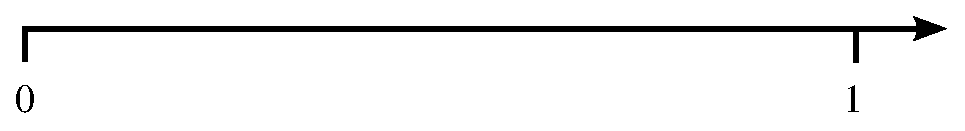
\includegraphics[width=10cm]{eps/interval.eps}
    \caption{The reference interval.}
    \label{fig:interval}
  \end{center}
\end{figure}

\begin{table}[H]
\linespread{1.2}\selectfont
  \begin{center}
    \begin{tabular}{|c|c|}
      \hline
      Vertex & Coordinate \\
      \hline
      \hline
      $v_0$ & $x = 0$ \\
      \hline
      $v_1$ & $x = 1$ \\
      \hline
    \end{tabular}
    \caption{Vertex coordinates of the reference interval.}
    \label{tab:interval,vertices}
  \end{center}
\end{table}

\newpage
\section{The reference triangle}

The reference triangle is shown in Figure~\ref{fig:triangle} and is
defined by its three vertices with coordinates as specified in
Table~\ref{tab:triangle,vertices}.

\begin{figure}[H]
  \begin{center}
    \psfrag{v0}{$(0, 0)$}
    \psfrag{v1}{$(1, 0)$}
    \psfrag{v2}{$(0, 1)$}
    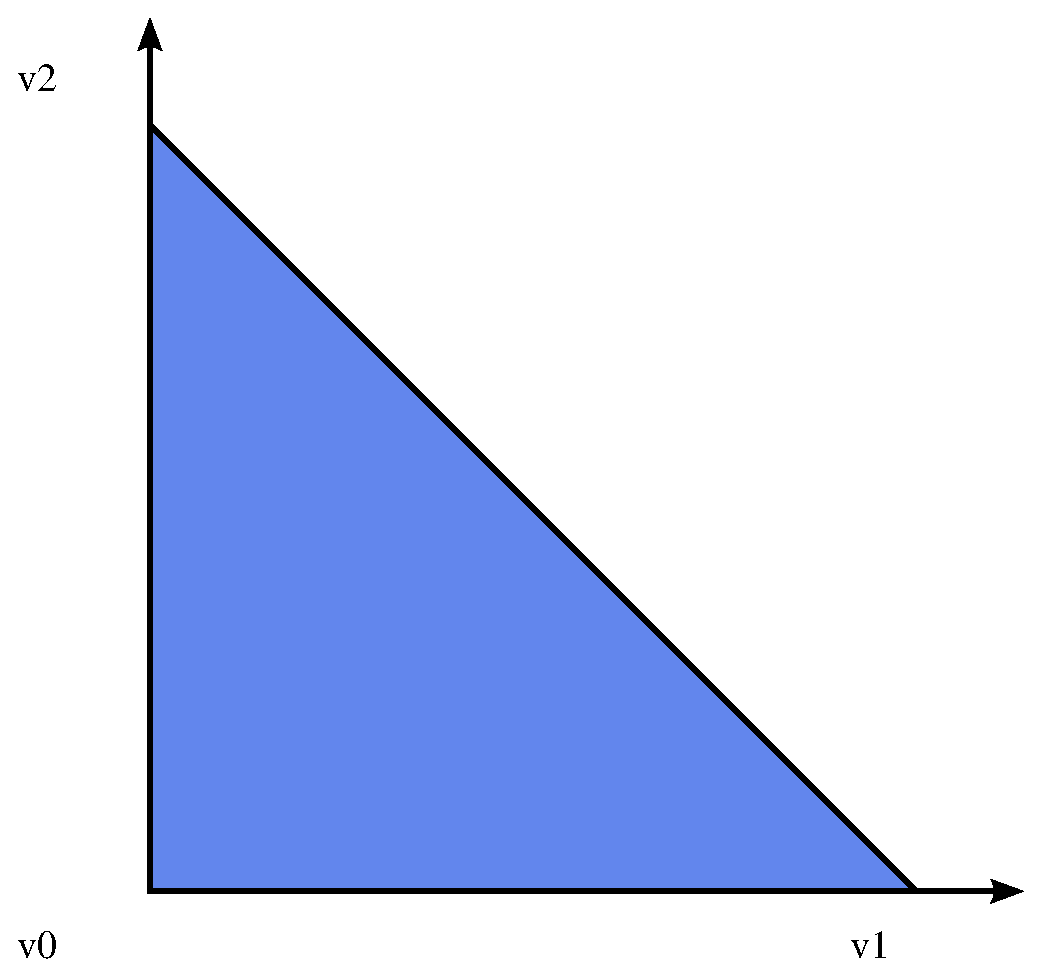
\includegraphics[width=8cm]{eps/triangle.eps}
    \caption{The reference triangle.}
    \label{fig:triangle}
  \end{center}
\end{figure}

\begin{table}[H]
\linespread{1.2}\selectfont
  \begin{center}
    \begin{tabular}{|c|c|}
      \hline
      Vertex & Coordinate \\
      \hline
      \hline
      $v_0$ & $x = (0, 0)$ \\
      \hline
      $v_1$ & $x = (1, 0)$ \\
      \hline
      $v_2$ & $x = (0, 1)$ \\
      \hline
    \end{tabular}
    \caption{Vertex coordinates of the reference triangle.}
    \label{tab:triangle,vertices}
  \end{center}
\end{table}

\newpage
\section{The reference quadrilateral}

The reference quadrilateral is shown in Figure~\ref{fig:quadrilateral}
and is defined by its four vertices with coordinates as specified in
Table~\ref{tab:quadrilateral,vertices}.

\begin{figure}[H]
  \begin{center}
    \psfrag{v0}{$(0, 0)$}
    \psfrag{v1}{$(1, 0)$}
    \psfrag{v2}{$(1, 1)$}
    \psfrag{v3}{$(0, 1)$}
    \includegraphics[width=8cm]{eps/quadrilateral.eps}
    \caption{The reference quadrilateral.}
    \label{fig:quadrilateral}
  \end{center}
\end{figure}

\begin{table}[H]
\linespread{1.2}\selectfont
  \begin{center}
    \begin{tabular}{|c|c|}
      \hline
      Vertex & Coordinate \\
      \hline
      \hline
      $v_0$ & $x = (0, 0)$ \\
      \hline
      $v_1$ & $x = (1, 0)$ \\
      \hline
      $v_2$ & $x = (1, 1)$ \\
      \hline
      $v_3$ & $x = (0, 1)$ \\
      \hline
    \end{tabular}
    \caption{Vertex coordinates of the reference quadrilateral.}
    \label{tab:quadrilateral,vertices}
  \end{center}
\end{table}

\newpage
\section{The reference tetrahedron}

The reference tetrahedron is shown in Figure~\ref{fig:tetrahedron} and
is defined by its four vertices with coordinates as specified in
Table~\ref{tab:tetrahedron,vertices}.

\begin{figure}[H]
  \begin{center}
    \psfrag{v0}{$(0, 0, 0)$}
    \psfrag{v1}{$(1, 0, 0)$}
    \psfrag{v2}{$(0, 1, 0)$}
    \psfrag{v3}{$(0, 0, 1)$}
    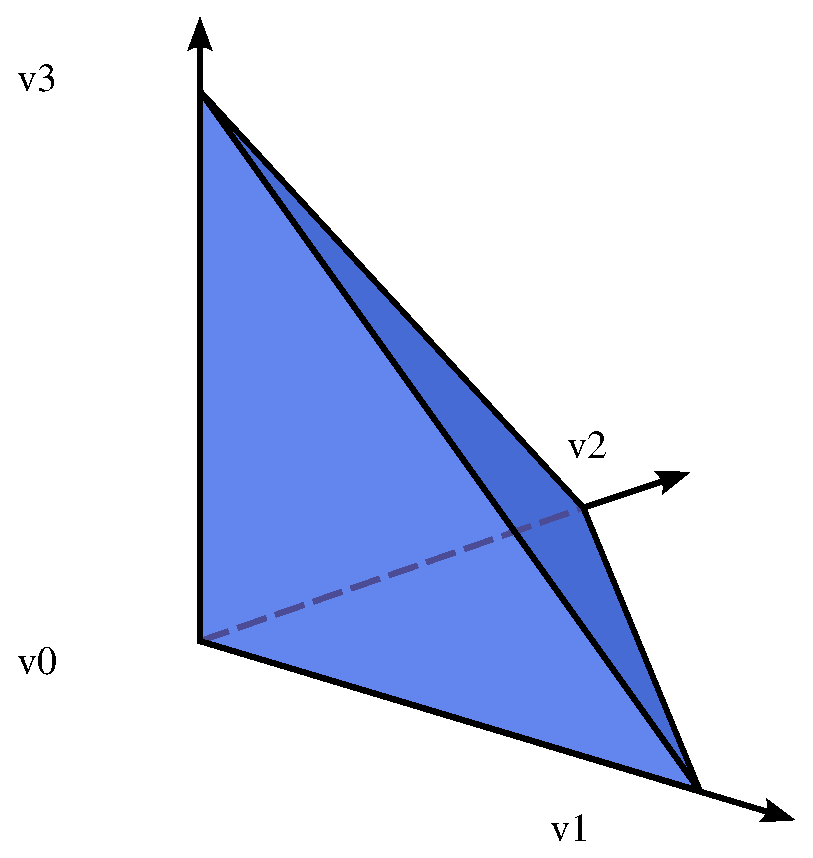
\includegraphics[width=6cm]{eps/tetrahedron.eps}
    \caption{The reference tetrahedron.}
    \label{fig:tetrahedron}
  \end{center}
\end{figure}

\begin{table}[H]
\linespread{1.2}\selectfont
  \begin{center}
    \begin{tabular}{|c|c|}
      \hline
      Vertex & Coordinate \\
      \hline
      \hline
      $v_0$ & $x = (0, 0, 0)$ \\
      \hline
      $v_1$ & $x = (1, 0, 0)$ \\
      \hline
      $v_2$ & $x = (0, 1, 0)$ \\
      \hline
      $v_3$ & $x = (0, 0, 1)$ \\
      \hline
    \end{tabular}
    \caption{Vertex coordinates of the reference tetrahedron.}
    \label{tab:tetrahedron,vertices}
  \end{center}
\end{table}

\newpage
\section{The reference hexahedron}

The reference hexahedron is shown in Figure~\ref{fig:hexahedron} and
is defined by its eight vertices with coordinates as specified in
Table~\ref{tab:hexahedron,vertices}.

\begin{figure}[H]
\linespread{1.2}\selectfont
  \begin{center}
    \psfrag{v0}{$(0, 0, 0)$}
    \psfrag{v1}{$(1, 0, 0)$}
    \psfrag{v2}{$(1, 1, 0)$}
    \psfrag{v3}{$(0, 1, 0)$}
    \psfrag{v4}{$(0, 0, 1)$}
    \psfrag{v5}{$(1, 0, 1)$}
    \psfrag{v6}{$(1, 1, 1)$}
    \psfrag{v7}{$(0, 1, 1)$}
    \includegraphics[width=9cm]{eps/hexahedron.eps}
    \caption{The reference hexahedron.}
    \label{fig:hexahedron}
  \end{center}
\end{figure}

\begin{table}[H]
\linespread{1.2}\selectfont
  \begin{center}
    \begin{tabular}{|c|c|}
      \hline
      Vertex & Coordinate \\
      \hline
      \hline
      $v_0$ & $x = (0, 0, 0)$ \\
      \hline
      $v_1$ & $x = (1, 0, 0)$ \\
      \hline
      $v_2$ & $x = (1, 1, 0)$ \\
      \hline
      $v_3$ & $x = (0, 1, 0)$ \\
      \hline
    \end{tabular}
    \begin{tabular}{|c|c|}
      \hline
      Vertex & Coordinate \\
      \hline
      \hline
      $v_4$ & $x = (0, 0, 1)$ \\
      \hline
      $v_5$ & $x = (1, 0, 1)$ \\
      \hline
      $v_6$ & $x = (1, 1, 1)$ \\
      \hline
      $v_7$ & $x = (0, 1, 1)$ \\
      \hline
    \end{tabular}
    \caption{Vertex coordinates of the reference hexahedron.}
    \label{tab:hexahedron,vertices}
  \end{center}
\end{table}


\chapter{Numbering of mesh entities}

The numbering of mesh entities used in DOLFIN follows the
UFC specification~\cite{www:UFC} for each mesh that has been ordered.\footnote{To order a mesh, call the \texttt{order()} function: \texttt{mesh.order()}.}
\input{chapters/numbering_common}

\chapter{Design}

This chapter discusses details of the design of \dolfin{} and is
intended mainly for developers of \dolfin{}.

\section{Linear algebra}

The linear algebra library provides a uniform interface to uBlas
and PETSc linear algebra through a set of wrappers for basic data
structures (matrices and vectors) and solvers, such as Krylov subspace
solvers with preconditioners.

For both sets of wrappers, a common interface is defined by the
classes \texttt{GenericMatrix} and \texttt{GenericVector}. \dolfin{}
provides a number of algorithms, most notably the assembly algorithms,
that work only through the common interface, which means that these
algorithms work for any given representation that implements the
interface specified by \texttt{GenericMatrix} or
\texttt{GenericVector}. A class diagram for the \dolfin{} linear
algebra implementation is given in Figure~\ref{fig:laclasses}.

\begin{figure}[htbp]
  \begin{center}
    \includegraphics[width=0.95\textwidth]{eps/class-diagram-la.eps}
    \caption{Class diagram of the linear algebra classes in \dolfin{}.}
    \label{fig:laclasses}
  \end{center}
\end{figure}


\input{chapters/installation.tex}
\chapter{Contributing code}
\index{contributing}

If you have created a new module, fixed a bug somewhere, or have made
a small change which you want to contribute to \dolfin{}, then the
best way to do so is to send us your contribution in the form of a
patch. A patch is a file which describes how to transform a file or
directory structure into another. The patch is built by comparing a
version which both parties have against the modified version which
only you have.

%------------------------------------------------------------------------------
\section{Creating a patch}
\index{diff}
\index{patch}

The tool used to create a patch is called \texttt{diff} and the tool
used to apply the patch is called \texttt{patch}. These tools are free
software and are standard on most Unix systems.

Here's an example of how it works. Start from the latest release of
\dolfin{}, which we here assume is release 0.5.0. You then have a
directory structure under \texttt{dolfin-0.5.0} where you have made
modifications to some files which you think could be useful to
other users.

\begin{enumerate}
\item
  Clean up your modified directory structure to remove temporary and binary
  files which will be rebuilt anyway:
  \begin{verbatim}
    # make clean
  \end{verbatim}
\item
  From the parent directory, rename the \dolfin{} directory to something else:
  \begin{verbatim}
    # mv dolfin-0.5.0 dolfin-0.5.0-mod
  \end{verbatim}
\item
  Unpack the version of \dolfin{} that you started from:
  \begin{verbatim}
    # tar zxfv dolfin-0.5.0.tar.gz
  \end{verbatim}
\item
  You should now have two \dolfin{} directory structures in your current directory:
  \begin{verbatim}
    # ls
    dolfin-0.5.0
    dolfin-0.5.0-mod
  \end{verbatim}
\item
  Now use the \texttt{diff} tool to create the patch:
  \begin{verbatim}
    # diff -u --new-file --recursive dolfin-0.5.0
      dolfin-0.5.0-mod > dolfin-<identifier>-<date>.patch
  \end{verbatim}
  written as one line, where \texttt{<identifier>} is a keyword that
  can be used to identify the patch as coming from you (your username,
  last name, first name, a nickname etc) and \texttt{<date>} is
  today's date in the format \texttt{yyyy-mm-dd}.
\item
  The patch now exists as \texttt{dolfin-<identifier>-<date>.patch}
  and can be distributed to other people who already have
  \texttt{dolfin-0.5.0} to easily create your modified version. If the
  patch is large, compressing it with for example \texttt{gzip} is
  advisable:
  \begin{verbatim}
    # gzip dolfin-<identifier>-<date>.patch
  \end{verbatim}
\end{enumerate}

%------------------------------------------------------------------------------
\section{License agreement}
\index{license}

By contributing a patch to \dolfin{}, you agree to license your
contributed code under the GNU General Public License (a condition
also built into the GPL license of the code you have modified). Before
creating the patch, please update the author and date information of
the file(s) you have modified according to the following example:

\begin{verbatim}
  // Copyright (C) 2004-2005 Johan Hoffman and Anders Logg.
  // Licensed under the GNU GPL Version 2.
  //
  // Modified by Johan Jansson 2005.
  // Modified by Garth N. Wells 2005.
  //
  // First added:  2004-06-22
  // Last changed: 2005-09-01
\end{verbatim}

As a rule of thumb, the original author of a file holds the copyright.

%------------------------------------------------------------------------------
\section{Sending patches}
\index{patch}

Patch files should be sent to the \dolfin{} mailing list at the address
\begin{verbatim}
  dolfin-dev@fenics.org
\end{verbatim}
Include a short description of what your patch accomplishes. Small
patches have a better chance of being accepted, so if you are making a
major contribution, please consider breaking your changes up into
several small self-contained patches if possible.

%------------------------------------------------------------------------------
\section{Applying a patch (maintainers)}
\index{patch}

Let's say that a patch has been built relative to \dolfin{} release 0.5.0.
The following description then shows how to apply the patch to a clean
version of release 0.5.0.

\begin{enumerate}
\item
  Unpack the version of \dolfin{} which the patch is built relative to:
  \begin{verbatim}
    # tar zxfv dolfin-0.5.0.tar.gz
  \end{verbatim}
\item
  Check that you have the patch \texttt{dolfin-<identifier>-<date>.patch} and the \dolfin{}
  directory structure in the current directory:
  \begin{verbatim}
    # ls
    dolfin-0.5.0
    dolfin-<identifier>-<date>.patch
  \end{verbatim}
  Unpack the patch file using \texttt{gunzip} if necessary.
\item
  Enter the \dolfin{} directory structure:
  \begin{verbatim}
    # cd dolfin-0.5.0
  \end{verbatim}
\item
  Apply the patch:
  \begin{verbatim}
    # patch -p1 < ../dolfin-<identifier>-<date>.patch
  \end{verbatim}
  The option \texttt{-p1} strips the leading directory from the filename
  references in the patch, to match the fact that we are applying the
  patch from inside the directory. Another useful option to
  \texttt{patch} is \texttt{--dry-run} which can be used to test the
  patch without actually applying it.
\item
  The modified version now exists as \texttt{dolfin-0.5.0}.
\end{enumerate}

% DOLFIN-specific part of chapter contributing.tex

%------------------------------------------------------------------------------
\section{License agreement}
\index{license}

By contributing a patch to \package{}, you agree to license your
contributed code under the GNU General Public License (a condition
also built into the GPL license of the code you have modified). Before
creating the patch, please update the author and date information of
the file(s) you have modified according to the following example:

\begin{code}
// Copyright (C) 2004-2005 Johan Hoffman and Anders Logg.
// Licensed under the GNU LGPL Version 2.1.
//
// Modified by Johan Jansson 2005.
// Modified by Garth N. Wells 2005.
//
// First added:  2004-06-22
// Last changed: 2005-09-01
\end{code}

As a rule of thumb, the original author of a file holds the copyright.

\chapter{Contributors}

\devnote{List all contributors here.}
\input{chapters/license.tex}

\end{document}
